
\chapter{Unit Conversion}


Extracted from~\cite{Balmer_Book}:\\
  \begin{tabular}{c l}
     \hspace{1cm} & R.T. Balmer \\
                  & Modern Engineering Thermodynamics \\
                  & Academic Press, 2011  \\
  \end{tabular}


\begin{list}{\bf Example \arabic{qcounter}:~}{\usecounter{qcounter}}
%
   \item\label{Example:UnitConversion1} Calculate the volume $\left(\text{in m}^{3}\right)$ of 1 kg of hydrogen gas $\left(\text{molecular mass of 2.016 kg.kgmol}^{-1}\right)$ at 27$^{\circ}$C and 1 bar. Assume ideal gas behaviour.
     \begin{description}
        \item[Solution:] We can use the ideal gas equation of state to calculate the volume of H$_{2}$ gas,
           \begin{displaymath}
              V = \frc{nRT}{P},
           \end{displaymath}
           where $n = m/MW$ is the number of moles, $m$, $MW$ and $R$ are the mass, molecular mass, and universal gas constant, respectively. We should be able to replace the variables with their values,
           \begin{eqnarray}
              V &=& \frc{nRT}{P} = \frc{ \frc{m}{MW} R T }{ P } \nonumber \\
                &=& \frc{ \frc{ 1\text{ kg}}{ 2.016\text{ kg.kgmol}^{-1}}\;\; 0.08314\frc{\text{bar.m}^{3}}{\text{kgmol.K}}\;\; ( 27 + 273.15)\text{ K}}{ 1 \text{ bar}},\nonumber
           \end{eqnarray}
           It is clear that the units above are consistent and can be easily eliminated resulting in m$^{3}$,
           \begin{eqnarray}
              V &=& \frc{ \frc{ 1\cancel{\text{ kg}}}{ 2.016\text{ \cancel{kg}.}\cancel{\text{kgmol}^{-1}}}\;\; 0.08314\frc{\text{\cancel{bar}.m}^{3}}{\text{\cancel{kgmol}.\cancel{K}}}\;\; ( 27 + 273.15)\cancel{\text{ K}}}{ 1 \text{ \cancel{bar}}},\nonumber \\
                &=& 12.3782\text{ m}^{3}.\nonumber
           \end{eqnarray}

     \end{description}
%
   \item\label{Example:UnitConversion2}  Liquid water at 0.70 bar is transferred from a condenser to a boiler through a pump. The pressure in the exit of the pump is 25 bar. Assuming that the water undertakes an isentropic (\ie constant entropy) compression, calculate the specific enthalpy of the water after the pump. Consider that the liquid water as incompressible and
       \begin{displaymath}
          dh = Tds + vdP,
       \end{displaymath}
where h, s, v are specific enthalpy (kJ/kg), entropy (kJ/(kg.K)) and volume (m$^{3}$.kg).
     \begin{description}
        \item[Solution:] If the process is isentropic, therefore $ds=0$ and the fundamental thermodynamic relation is simplified to,
       \begin{displaymath}
          dh = vdP \Longrightarrow h_{2} - h_{1} = v\left(P_{2}-P_{1}\right),
       \end{displaymath}
      or summarising,
       \begin{center}
         \begin{tabular}{c| c c c}
            State  & $P$ (bar)  & $h$ (kJ/kg) & $v$ $\left(\text{m}^{3}\text{.kg}\right)$ \\
\hline
              1    &   0.70    &  376.70   &  1.0360$\times$10$^{-3}$                 \\
              2    &  25.0    & \red{h$_{2}$}& 1.0360$\times$10$^{-3}$ 
         \end{tabular}
       \end{center}
       Values of {\it State 1} were obtained from the water saturated table (Appendix~\ref{Appendix:Saturated_SH_Tables}). Note that as the fluid is assumed incompressible there is no variation in the volume, $v_{1}=v_{2}$.
       \begin{eqnarray}
         h_{2} &=& h_{1} = v\left(P_{2}-P_{1}\right) \nonumber \\
              &=& 376.70\frc{\text{kJ}}{\text{kg}} + 1.0360\times 10^{-3}\frc{\text{m}^{3}}{\text{kg}}\;\left(25 - 0.70\right)\text{ bar}  \nonumber\\
              &=& 376.70\frc{\text{kJ}}{\text{kg}} + 0.02517 \frc{\text{m}^{3}.\text{bar}}{\text{kg}} \nonumber
       \end{eqnarray}
       It is clear that the units in the two terms of the r.h.s. of the equation contain distinct units that \underline{can not} be summed up. Therefore, we need to convert $\left[\text{m}^{3}.\text{bar}\right]$ to $[\text{kJ}]$. Bearing in mind that 1 J = 1 N.m = 1 kg.m$^{2}$.s$^{-2}$, we first can convert $\left[\text{m}^{3}.\text{bar}\right]$ to $\left[\text{kg.m}^{2}.\text{s}^{-2}\right]$
       \begin{displaymath}
          1 \cancelto{\blue{\text{m}^{2}}}{\text{m}^{3}}.\red{\cancel{\text{bar}}} \times \frc{\red{10^{5}\cancel{\text{ Pa}}}}{\red{1 \cancel{\text{ bar}}}} \times \frc{\red{ 1 \text{ kg}/\left(\cancel{\blue{\text{m}}}.\text{s}^{2}\right)}}{\red{ 1 \cancel{\text{ Pa}}}} = 10^{5} \frac{\text{kg.m}^{2}}{\text{s}^{2}}
       \end{displaymath}
       Now, replacing the converted $\left[\text{m}^{3}.\text{bar}\right]$ term in the r.h.s. of the expression for $h_{2}$,
       \begin{eqnarray}
         h_{2} &=& 376.70\frc{\text{kJ}}{\text{kg}} + 0.02517 \frc{\text{m}^{3}.\text{bar}}{\text{kg}} \nonumber \\
              &=& 376.70\frc{\text{kJ}}{\text{kg}} + 0.02517 \frc{\cancel{\left(\text{m}^{3}.\text{bar}\right)}}{\text{kg}} \times \frc{10^{5} \frac{\text{kg.m}^{2}}{\text{s}^{2}}}{1 \cancel{\left(\text{m}^{3}.\text{bar}\right)}} \nonumber \\
              &=& 376.70\frc{\text{kJ}}{\text{kg}} + 2517 \frc{\cancelto{\red{\text{J}}}{\frac{\text{kg.m}^{2}}{\text{s}^{2}}}}{\text{kg}}\nonumber\\
              &=& 376.70\frc{\text{kJ}}{\text{kg}} + 2517 \frc{\text{J}}{\text{kg}} \nonumber
       \end{eqnarray}
       We still \underline{can not} sum the two terms in the r.h.s., as the first term involves $\left[\text{kJ/kg}\right]$ whereas the second term is $\left[\text{J/kg}\right]$, therefore
       \begin{eqnarray}
         h_{2} &=& 376.70\frc{\text{kJ}}{\text{kg}} + 2517 \frc{\text{J}}{\text{kg}} \nonumber\\
              &=& 376.70\frc{\text{kJ}}{\text{kg}} + 2517 \frc{\cancel{\text{J}}}{\text{kg}} \red{\times \frc{1\text{ kJ}}{1000 \cancel{\text{J}}}}\nonumber\\
              &=& 379.22 \frc{\text{kJ}}{\text{kg}}\nonumber
       \end{eqnarray}
       


     \end{description}
%
\end{list}

  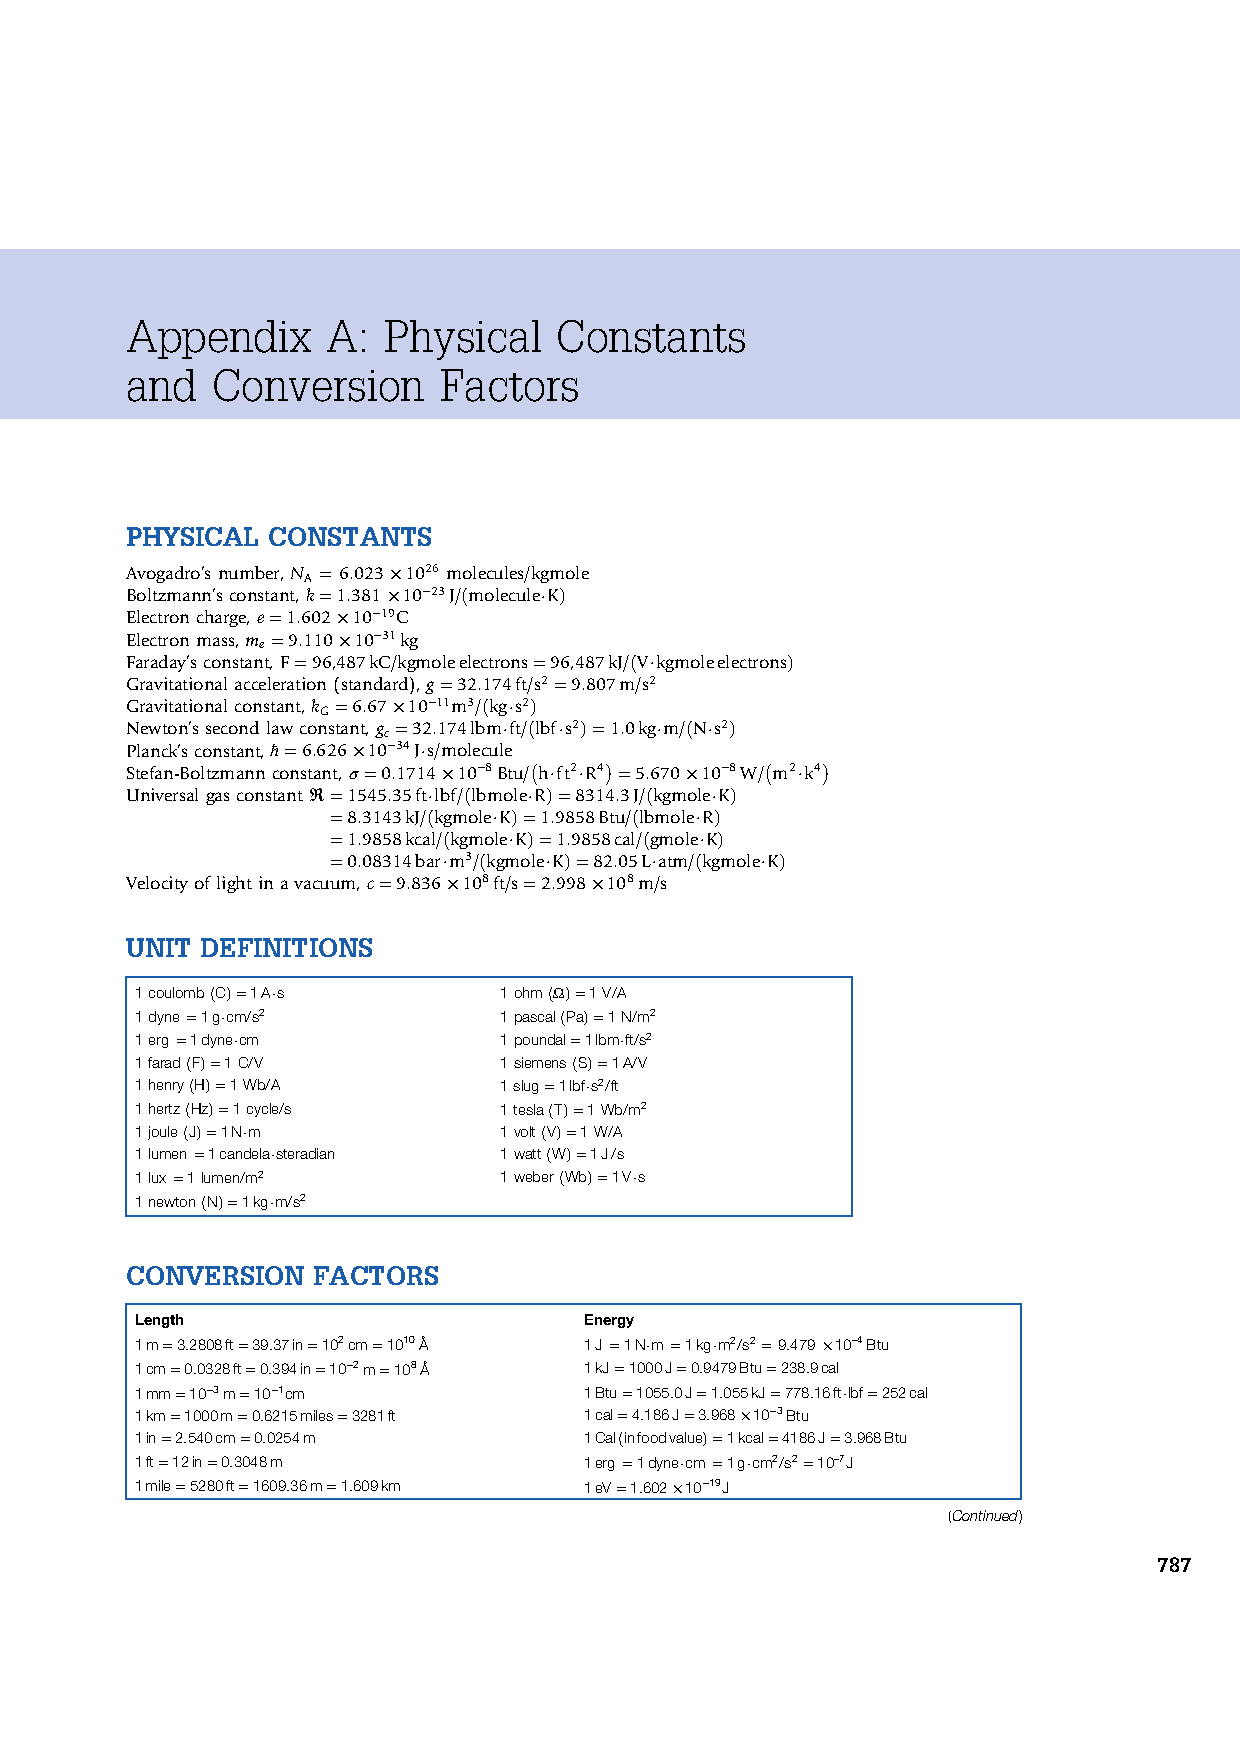
\includepdf[scale=1,pages=-,pagecommand={}, fitpaper]{./Pics/ChemEng_UnitConv.pdf}
